\documentclass[11pt]{beamer}
% \usetheme{Boadilla}
  \usetheme{default}


% acronyms for text or math mode
\newcommand {\ccast} {\mbox{\small CCAST}}
\newcommand {\cris} {\mbox{\small CrIS}}

\newcommand {\airs} {\mbox{\small AIRS}}
\newcommand {\iasi} {\mbox{\small IASI}}
\newcommand {\idps} {\mbox{\small IDPS}}
\newcommand {\nasa} {\mbox{\small NASA}}
\newcommand {\noaa} {\mbox{\small NOAA}}
\newcommand {\nstar} {\mbox{\small STAR}}
\newcommand {\umbc} {\mbox{\small UMBC}}
\newcommand {\uw}   {\mbox{\small UW}}

\newcommand {\fft}  {\mbox{\small FFT}}
\newcommand {\ifft} {\mbox{\small IFFT}}
\newcommand {\fir}  {\mbox{\small FIR}}
\newcommand {\fov}  {\mbox{\small FOV}}
\newcommand {\for}  {\mbox{\small FOR}}
\newcommand {\ict}  {\mbox{\small ICT}}
\newcommand {\ils}  {\mbox{\small ILS}}
\newcommand {\igm}  {\mbox{\small IGM}}
\newcommand {\opd}  {\mbox{\small OPD}}
\newcommand {\rms}  {\mbox{\small RMS}}
\newcommand {\zpd}  {\mbox{\small ZPD}}
\newcommand {\ppm}  {\mbox{\small PPM}}
\newcommand {\srf}  {\mbox{\small SRF}}
\newcommand {\sdr}  {\mbox{\small SDR}}

\newcommand {\ES} {\mbox{\small ES}}
\newcommand {\SP} {\mbox{\small SP}}
\newcommand {\IT} {\mbox{\small IT}}
\newcommand {\SA} {\mbox{\small SA}}

\newcommand {\ET} {\mbox{\small ET}}
\newcommand {\FT} {\mbox{\small FT}}

% abbreviations, mainly for math mode
\newcommand {\real} {\mbox{real}}
\newcommand {\imag} {\mbox{imag}}
\newcommand {\atan} {\mbox{atan}}
\newcommand {\obs}  {\mbox{obs}}
\newcommand {\calc} {\mbox{calc}}
\newcommand {\sinc} {\mbox{sinc}}
\newcommand {\psinc} {\mbox{psinc}}
\newcommand {\std} {\mbox{std}}

% symbols, for math mode only
\newcommand {\wnum} {\mbox{cm$^{-1}$}}
\newcommand {\lmax} {L_{\mbox{\tiny max}}}
\newcommand {\vmax} {V_{\mbox{\tiny max}}}

\newcommand {\tauobs} {\tau_{\mbox{\tiny obs}}}
\newcommand {\taucal} {\tau_{\mbox{\tiny calc}}}
\newcommand {\Vdc}  {V_{\mbox{\tiny DC}}}

\newcommand {\rIT} {r_{\mbox{\tiny\textsc{ict}}}}
\newcommand {\rES} {r_{\mbox{\tiny\textsc{es}}}}
\newcommand {\robs} {r_{\mbox{\tiny obs}}}

\newcommand {\rITobs} {r_{\mbox{\tiny\textsc{ict}}}^{\mbox{\tiny obs}}}
\newcommand {\rITcal} {r_{\mbox{\tiny\textsc{ict}}}^{\mbox{\tiny cal}}}

\newcommand {\ITmean} {\langle\mbox{\small IT}\rangle}
\newcommand {\SPmean} {\langle\mbox{\small SP}\rangle}


\title{CCAST and NOAA \\
  17--19 Feb 2015 SDR \\
  Algorithm Tests}
\author{H.~E.~Motteler, L.~L.~Strow}
\institute{
  UMBC Atmospheric Spectroscopy Lab \\
  Joint Center for Earth Systems Technology \\
}
\date{\today}
\begin{document}

%----------- slide --------------------------------------------------%
\begin{frame}[plain]
\titlepage
\end{frame}
%----------- slide --------------------------------------------------%
\begin{frame}
\frametitle{introduction}

\begin{itemize}

  \item we look at both relative and absolute comparisons of the
    17--19 Feb 2015 \ccast\ and \noaa\ high res {\sdr} test data

  \item although we looked at all four \noaa\ tests, we only show
    comparisons of {\ccast} with {\noaa} algorithm 4 and selected
    examples of algorithm~3

  \item supplemental slides include the \ccast\ calibration equation
    and notes on interpreting {\for} as sweep differences

  \item \ccast\ \sdr\ data from shortly after mission start is
    available online at asl.umbc.edu/pub/data/ccast.  See readme.txt
    for more information and ccast\_sdr.txt for the {\sdr} format
    specs

\end{itemize}

\end{frame}
%----------- slide --------------------------------------------------%
\begin{frame}
\frametitle{clear matchup tests}

\begin{itemize}

  \item start with 2400 clear matchups from the 17-19 Feb 2015 \\
    test data

  \item calculate upwelling radiances with kcarta at a 0.0025 cm-1
    grid and convolve to the {\cris} user grid

  \item calculate upwelling radiances with our IASI fast model and
    convolve to the {\cris} user grid

  \item compare calculated radiances with {\ccast} and with {\noaa}
    algorithm~4

  \item the convolutions from kcarta to \cris, {\iasi} to \cris, and
    the {\cris} sensor to user grid in {\ccast} are all done with
    double Fourier interpolation, with similar procedures and filters
    
\end{itemize}

\end{frame}
%----------- slide --------------------------------------------------%
\begin{frame}
\frametitle{clear matchup FOV and FOR distributions}
\begin{center}
  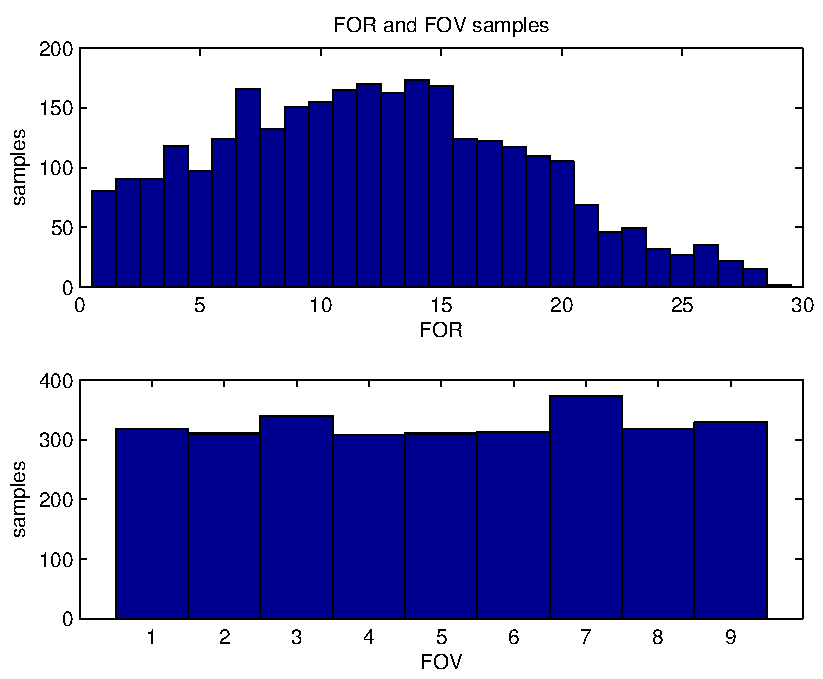
\includegraphics[scale=0.7]{figures/FOV_FOR_bins.pdf}
\end{center}
\end{frame}
%----------- slide --------------------------------------------------%
\begin{frame}
\frametitle{iasi sarta obs and obs minus calc}
\begin{center}
  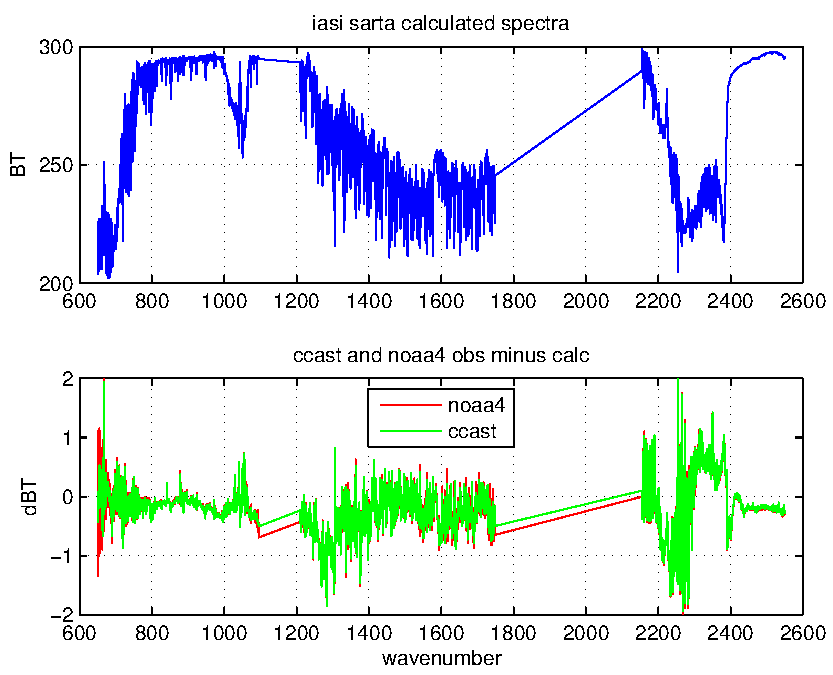
\includegraphics[scale=0.7]{figures/iasi_sarta_1.pdf}
\end{center}
\end{frame}
%----------- slide --------------------------------------------------%
\begin{frame}
\frametitle{iasi sarta obs minus calc details}
\begin{center}
  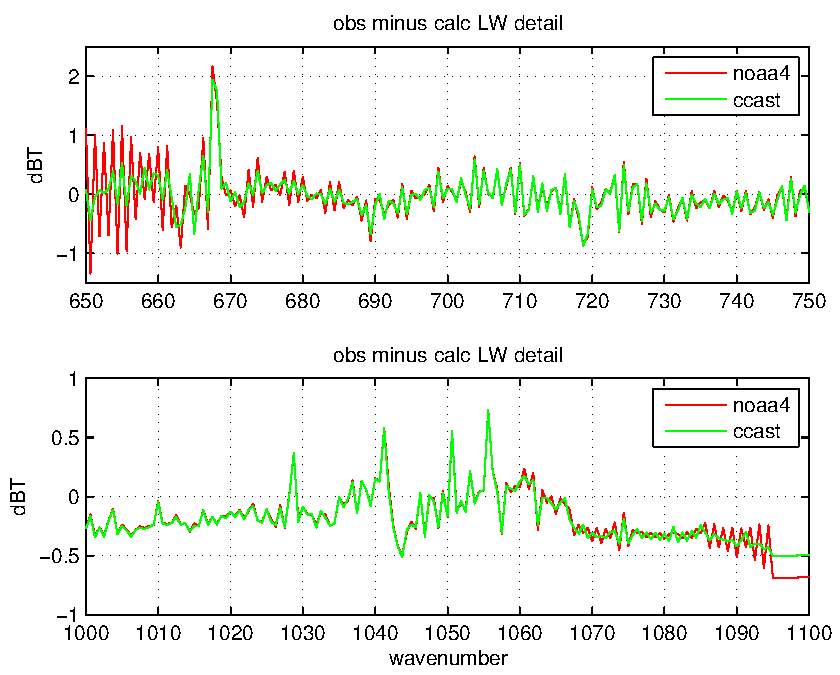
\includegraphics[scale=0.7]{figures/iasi_sarta_2.pdf}
\end{center}
\end{frame}
%----------- slide --------------------------------------------------%
\begin{frame}
\frametitle{iasi sarta obs minus calc details}
\begin{center}
  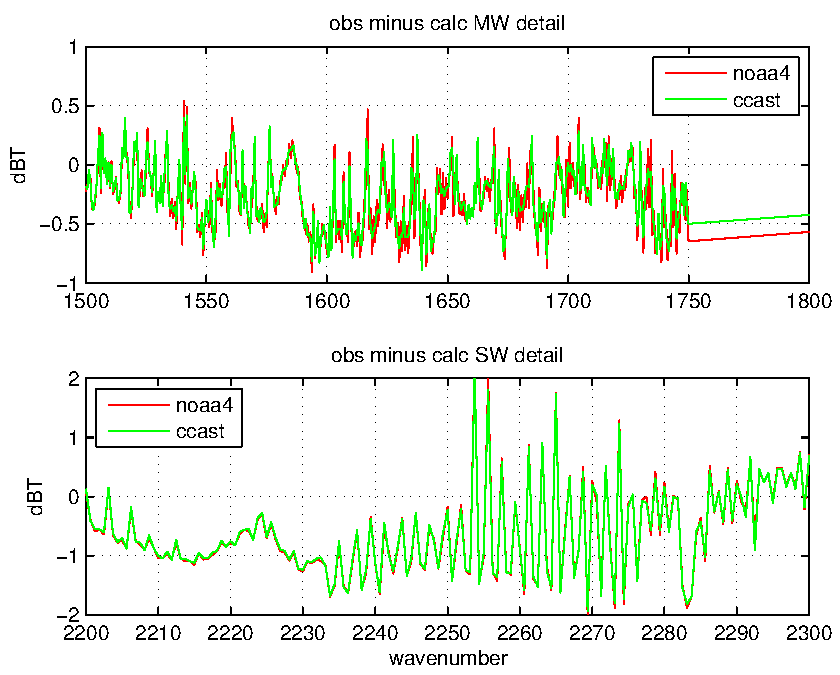
\includegraphics[scale=0.7]{figures/iasi_sarta_3.pdf}
\end{center}
\end{frame}
%----------- slide --------------------------------------------------%
\begin{frame}
\frametitle{kcarta obs minus calc}
\begin{center}
  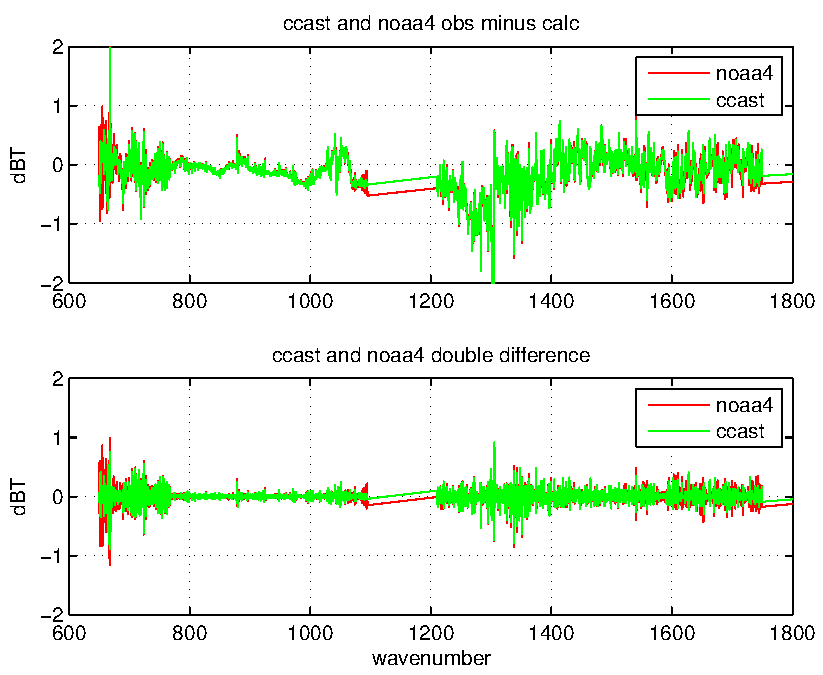
\includegraphics[scale=0.7]{figures/kcarta_all_1.pdf}
\end{center}
\end{frame}
%----------- slide --------------------------------------------------%
\begin{frame}
\frametitle{kcarta sweep differences}
\begin{center}
  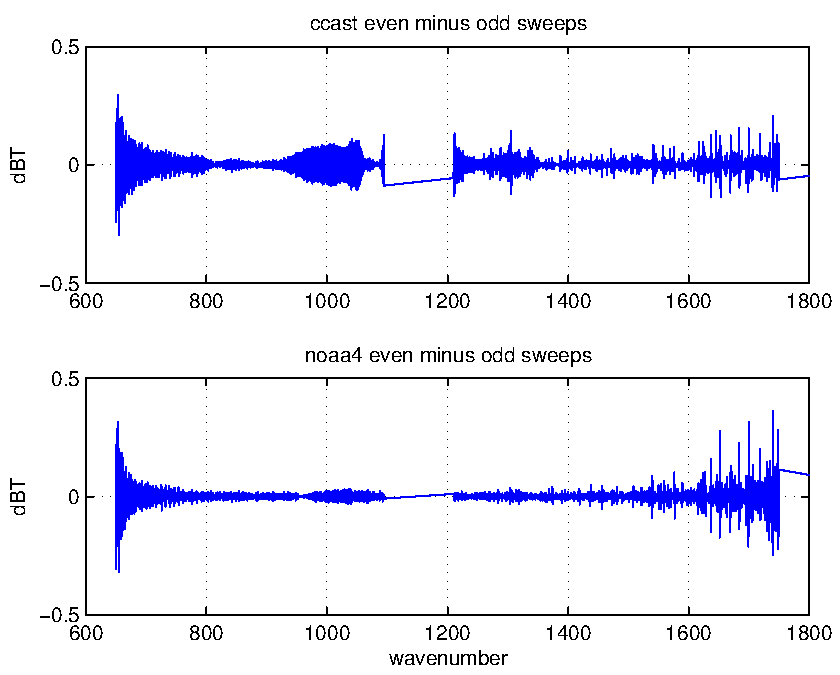
\includegraphics[scale=0.7]{figures/kcarta_all_2.pdf}
\end{center}
\end{frame}
%----------- slide --------------------------------------------------%
\begin{frame}
\frametitle{kcarta fov 1 obs minus calc}
\begin{center}
  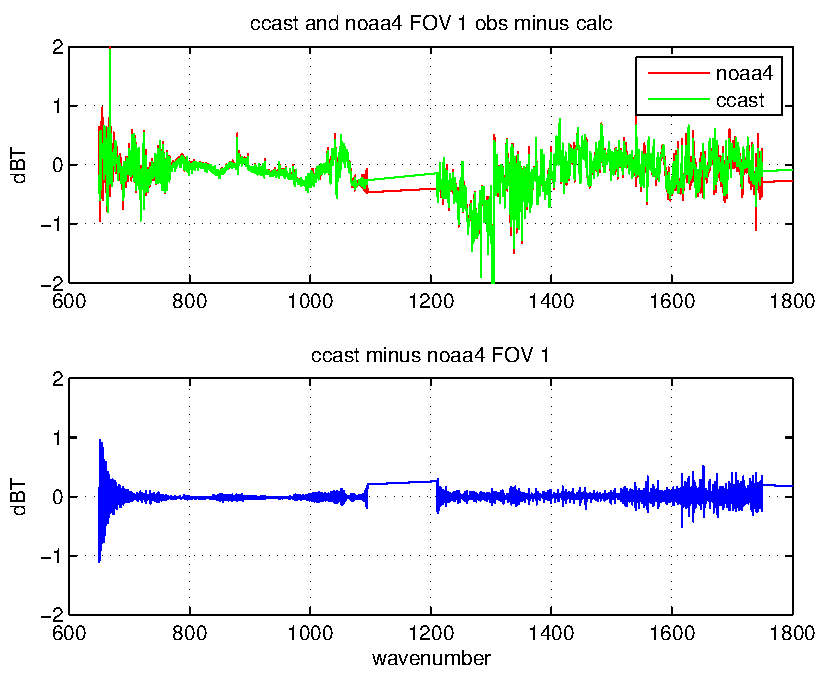
\includegraphics[scale=0.7]{figures/kcarta_FOV1.pdf}
\end{center}
\end{frame}
%----------- slide --------------------------------------------------%
\begin{frame}
\frametitle{kcarta fov 2 obs minus calc}
\begin{center}
  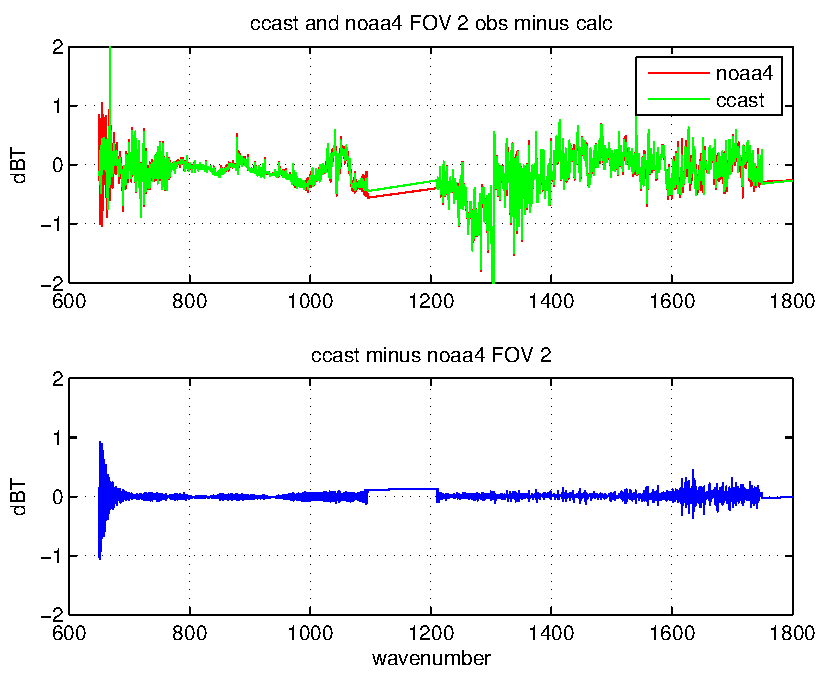
\includegraphics[scale=0.7]{figures/kcarta_FOV2.pdf}
\end{center}
\end{frame}
%----------- slide --------------------------------------------------%
\begin{frame}
\frametitle{kcarta fov 5 obs minus calc}
\begin{center}
  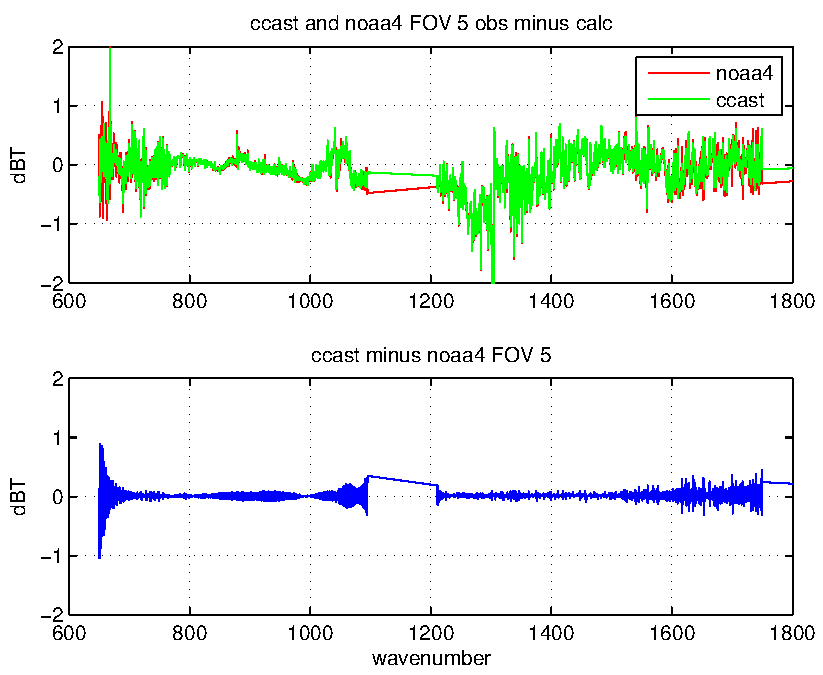
\includegraphics[scale=0.7]{figures/kcarta_FOV5.pdf}
\end{center}
\end{frame}
%----------- slide --------------------------------------------------%
\begin{frame}
\frametitle{clear matchup comments}

\begin{itemize}

  \item the {\ccast} obs minus calc residuals were consistently
    smaller than {\noaa} algorithm~4.

  \item the {\ccast} {\iasi} sarta residuals were much smaller at
    the LW band edges.  Due to {\iasi} starting at 645 cm-1, the
    wings of the filter used for convolving {\iasi} to {\cris} were
    narrower than those used for regular {\ccast} processing
    
  \item the {\noaa} algorithm 4 sweep differences were better overall,
    though slightly worse at the high end of the MW band
    
  \item we need to look at sweep differences broken out by {\fov}

\end{itemize}

\end{frame}
%----------- slide --------------------------------------------------%
\begin{frame}
\frametitle{relative test methods}

\begin{itemize}

  \item start with \ccast\ and \noaa\ high res {\sdr} data for the
    17--19 Feb 2015 tests

  \item take the average and standard deviation of \for\ 15 and 16
    together over the test period for each \fov, descending only,
    and compare with \fov\ 5

  \item take average of \for\ 15 and 16 separately over the test
    period for each \fov, descending only, filter to reduce scan
    geometry effects, and compare sweep directions
    
  \item ccast performance was similar to or better than {\noaa} for
    algorithms 1 and~2.  We compare ccast with {\noaa} algorithm 4
    and selected examples of algorithm~3
    
\end{itemize}

\end{frame}
%----------- slide --------------------------------------------------%
\begin{frame}
\frametitle{ccast sw relative to fov 5}
\begin{center}
  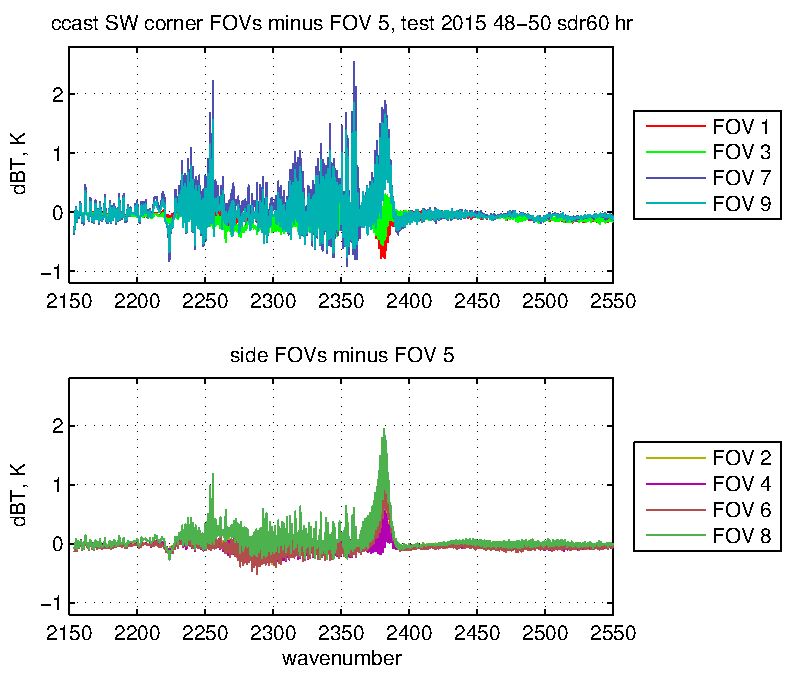
\includegraphics[scale=0.7]{figures/ccast_SW_dif_2015_48-50_sdr60_hr.pdf}
\end{center}
\end{frame}
%----------- slide --------------------------------------------------%
\begin{frame}
\frametitle{noaa 4 sw relative to fov 5}
\begin{center}
  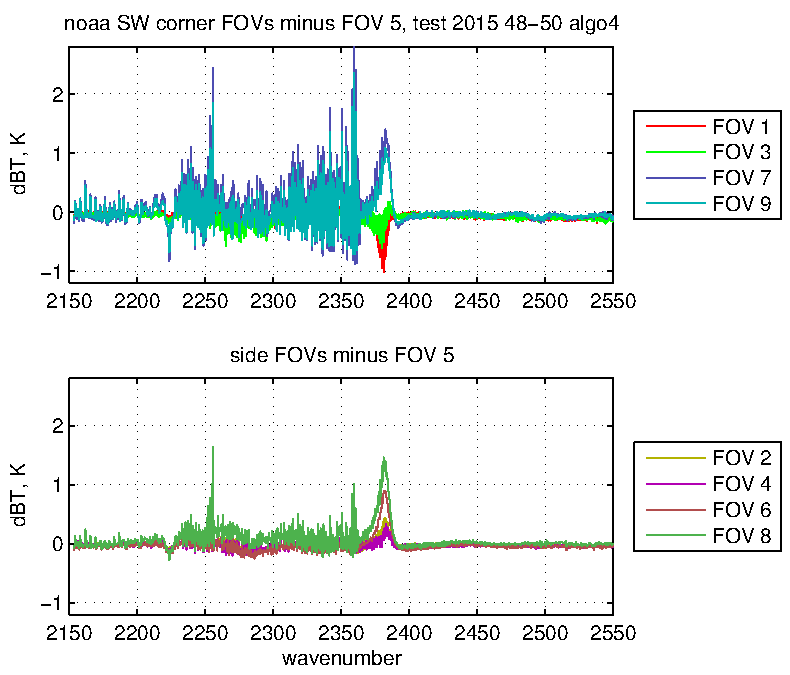
\includegraphics[scale=0.7]{figures/noaa_SW_dif_2015_48-50_algo4.pdf}
\end{center}
\end{frame}
%----------- slide --------------------------------------------------%
\begin{frame}
\frametitle{ccast sw sweep double difference}
\begin{center}
  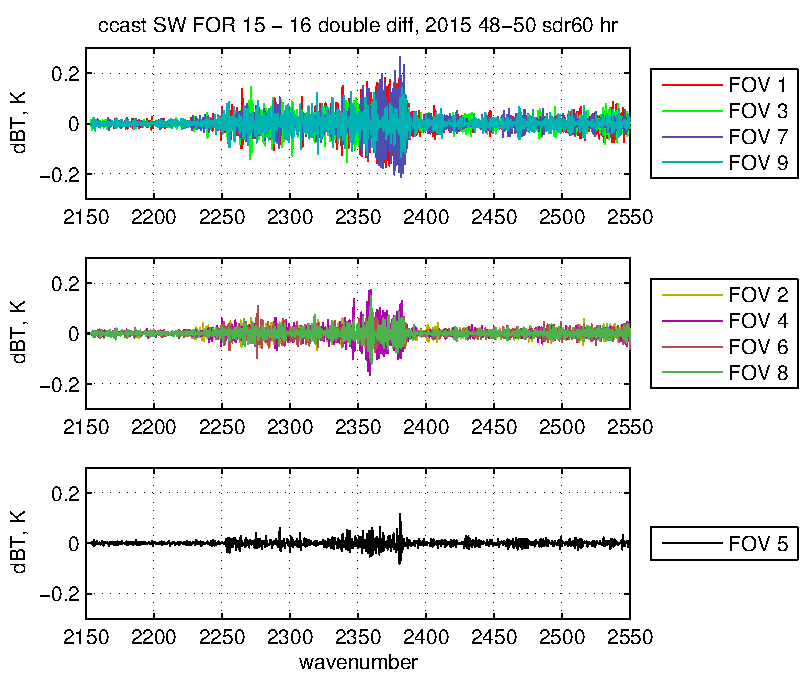
\includegraphics[scale=0.7]{figures/ccast_SW_sfil_2015_48-50_sdr60_hr.pdf}
\end{center}
\end{frame}
%----------- slide --------------------------------------------------%
\begin{frame}
\frametitle{noaa 3 sw sweep double difference}
\begin{center}
  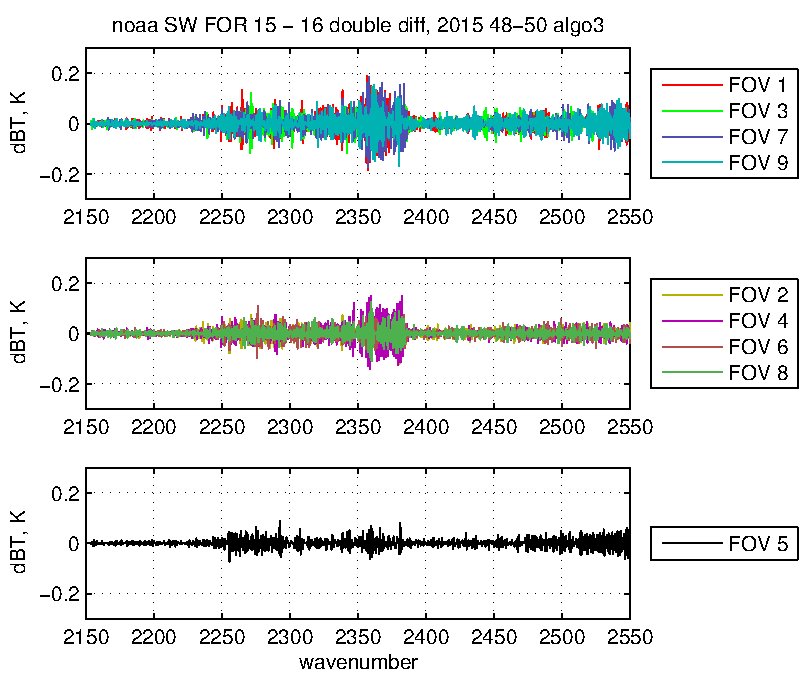
\includegraphics[scale=0.7]{figures/noaa_SW_sfil_2015_48-50_algo3.pdf}
\end{center}
\end{frame}
%----------- slide --------------------------------------------------%
\begin{frame}
\frametitle{noaa 4 sw sweep double difference}
\begin{center}
  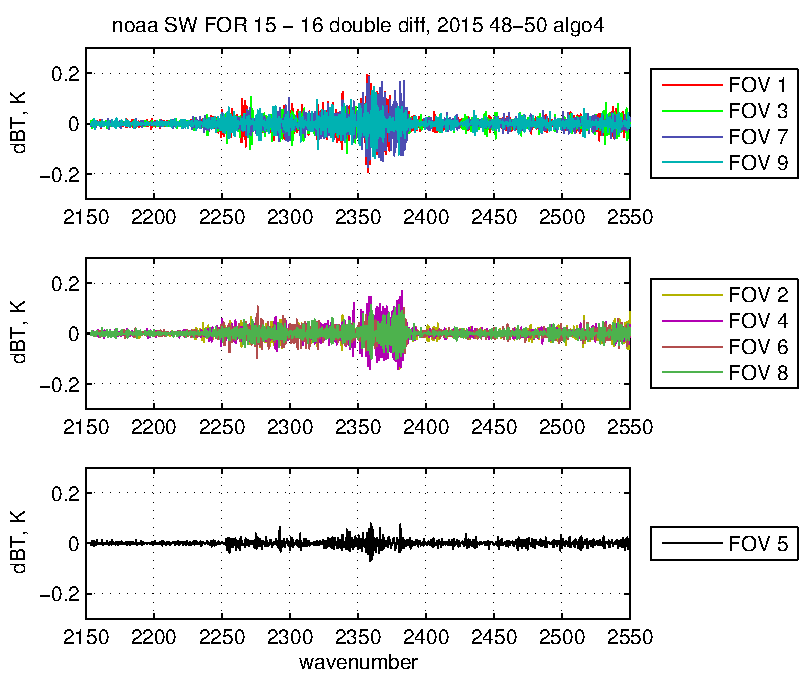
\includegraphics[scale=0.7]{figures/noaa_SW_sfil_2015_48-50_algo4.pdf}
\end{center}
\end{frame}
%----------- slide --------------------------------------------------%
\begin{frame}
\frametitle{ccast mw relative to FOV 5}
\begin{center}
  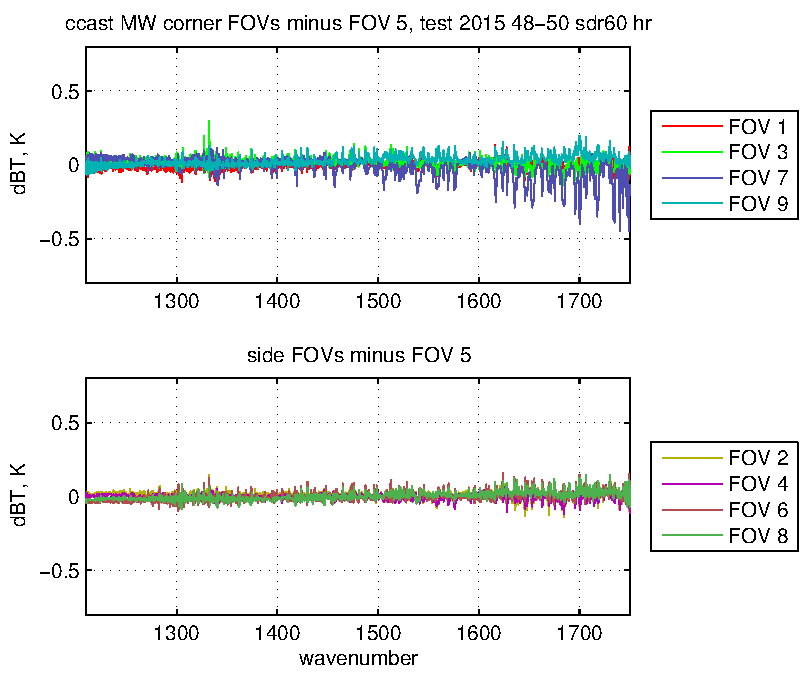
\includegraphics[scale=0.7]{figures/ccast_MW_dif_2015_48-50_sdr60_hr.pdf}
\end{center}
\end{frame}
%----------- slide --------------------------------------------------%
\begin{frame}
\frametitle{noaa 4 mw relative to fov 5}
\begin{center}
  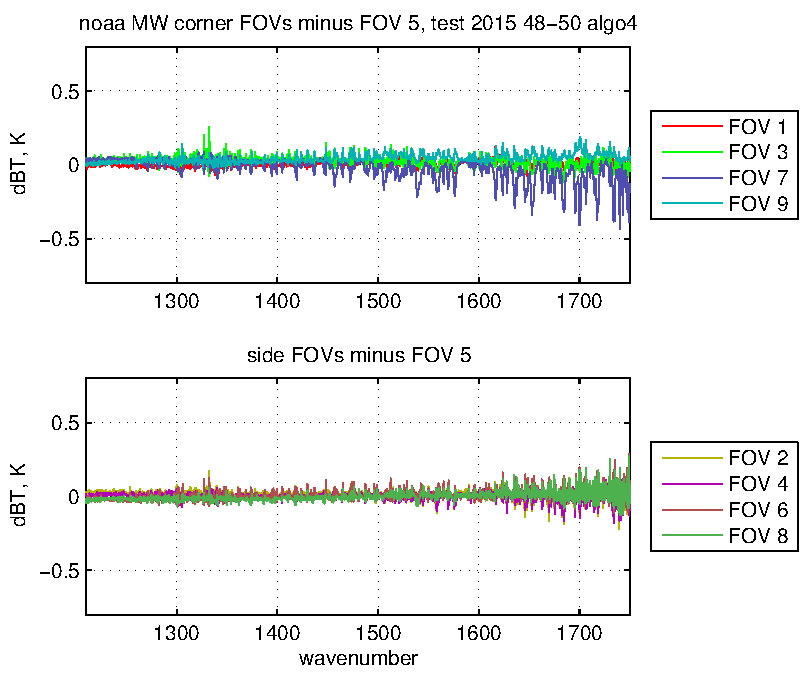
\includegraphics[scale=0.7]{figures/noaa_MW_dif_2015_48-50_algo4.pdf}
\end{center}
\end{frame}
%----------- slide --------------------------------------------------%
\begin{frame}
\frametitle{ccast mw sweep double difference}
\begin{center}
  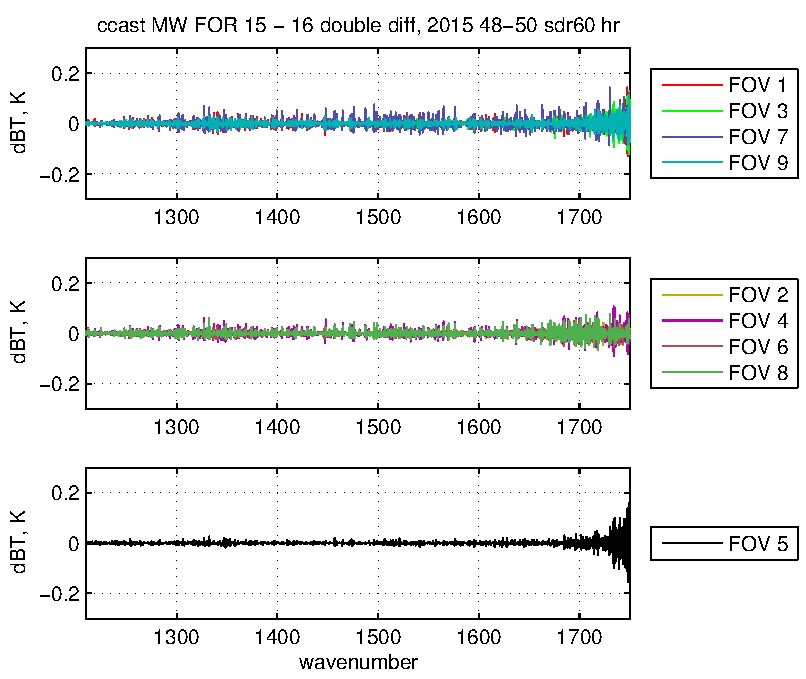
\includegraphics[scale=0.7]{figures/ccast_MW_sfil_2015_48-50_sdr60_hr.pdf}
\end{center}
\end{frame}
%----------- slide --------------------------------------------------%
\begin{frame}
\frametitle{noaa 4 mw sweep double difference}
\begin{center}
  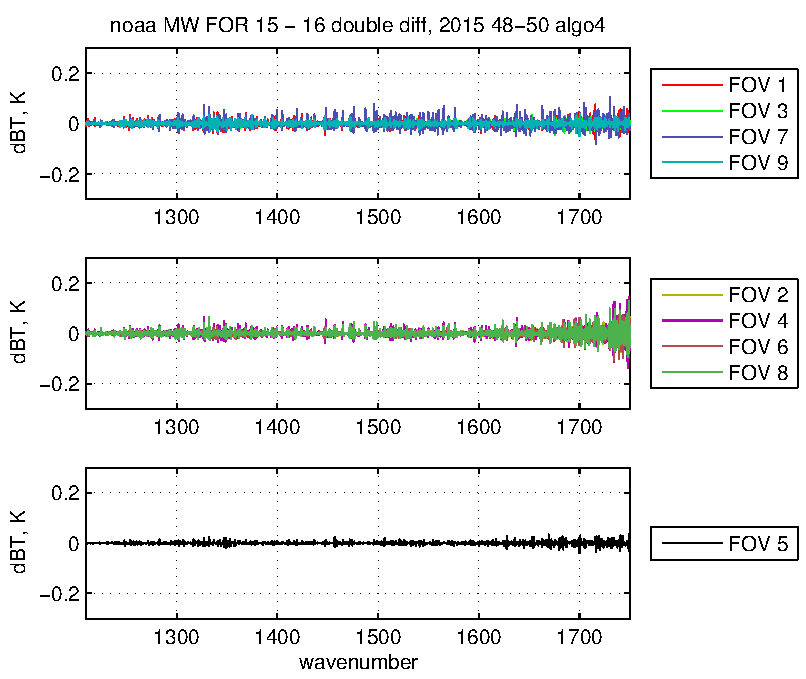
\includegraphics[scale=0.7]{figures/noaa_MW_sfil_2015_48-50_algo4.pdf}
\end{center}
\end{frame}
%----------- slide --------------------------------------------------%
\begin{frame}
\frametitle{ccast lw relative to fov 5}
\begin{center}
  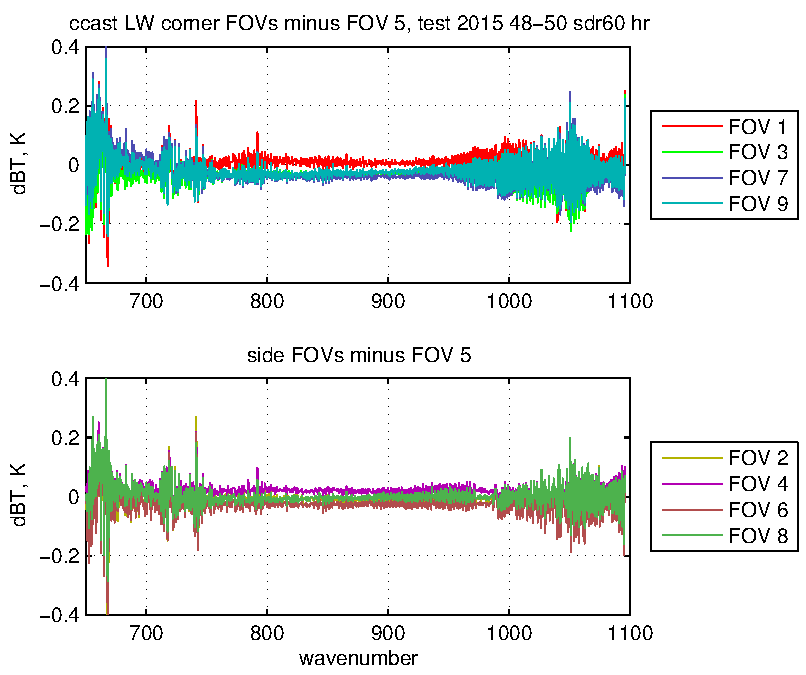
\includegraphics[scale=0.7]{figures/ccast_LW_dif_2015_48-50_sdr60_hr.pdf}
\end{center}
\end{frame}
%----------- slide --------------------------------------------------%
\begin{frame}
\frametitle{noaa 4 lw relative to fov 5}
\begin{center}
  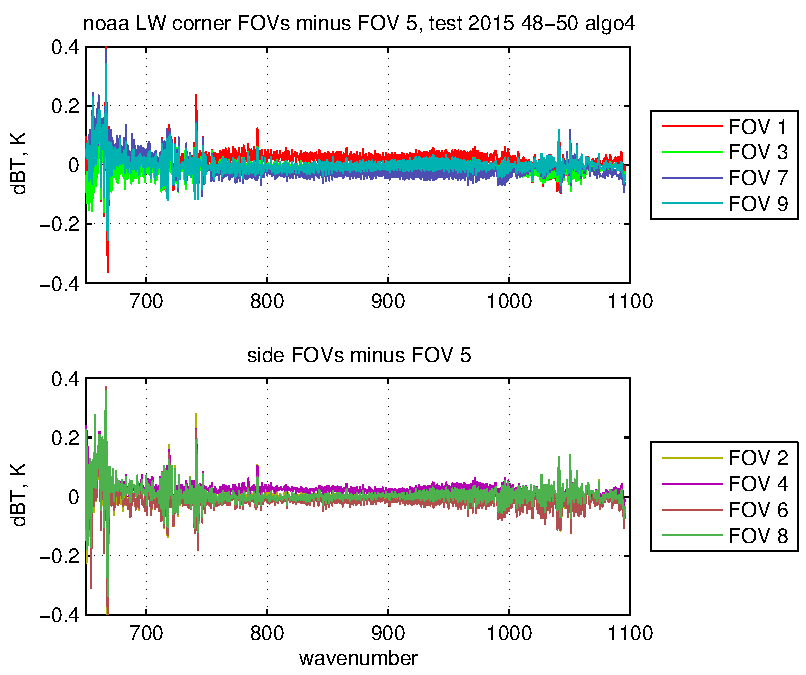
\includegraphics[scale=0.7]{figures/noaa_LW_dif_2015_48-50_algo4.pdf}
\end{center}
\end{frame}
%----------- slide --------------------------------------------------%
\begin{frame}
\frametitle{ccast lw sweep double difference}
\begin{center}
  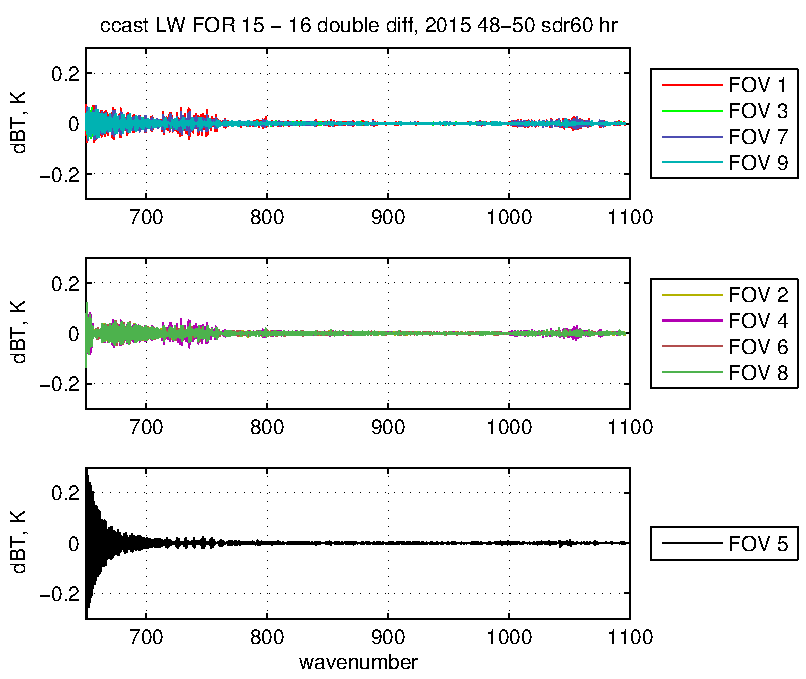
\includegraphics[scale=0.7]{figures/ccast_LW_sfil_2015_48-50_sdr60_hr.pdf}
\end{center}
\end{frame}
%----------- slide --------------------------------------------------%
\begin{frame}
\frametitle{noaa 3 lw sweep double difference}
\begin{center}
  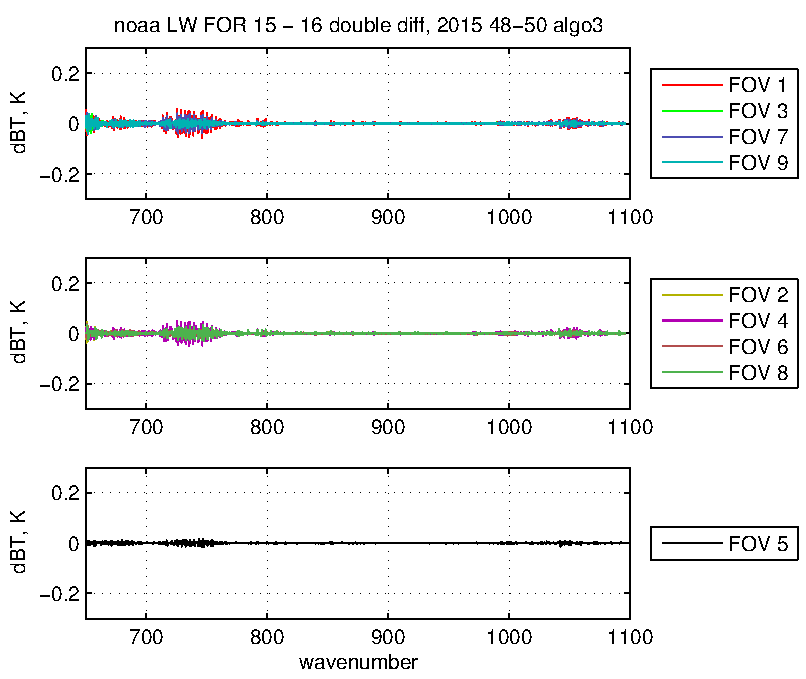
\includegraphics[scale=0.7]{figures/noaa_LW_sfil_2015_48-50_algo3.pdf}
\end{center}
\end{frame}
%----------- slide --------------------------------------------------%
\begin{frame}
\frametitle{noaa 4 lw sweep double difference}
\begin{center}
  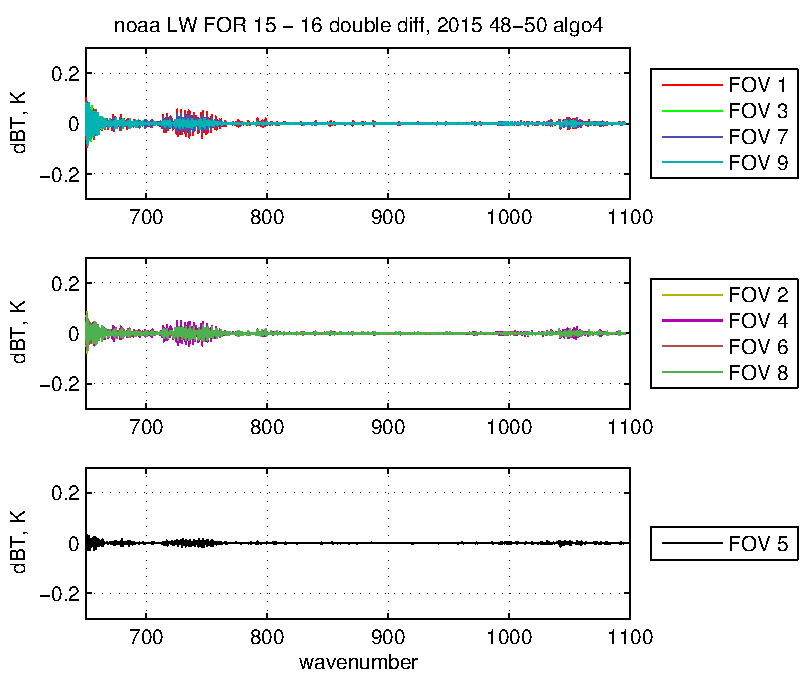
\includegraphics[scale=0.7]{figures/noaa_LW_sfil_2015_48-50_algo4.pdf}
\end{center}
\end{frame}
%----------- slide --------------------------------------------------%
\begin{frame}
\frametitle{relative test comments}

\begin{itemize}

  \item for the SW, {\noaa} 3 and 4 were similar or slightly better
    than {\ccast}.  For the MW results were similar, with {\ccast}
    slightly better for the FOV 5 relative test and {\noaa} for the
    sweep differences

  \item for the LW, {\noaa} 3 and 4 were significantly better than
    {\ccast}.  {\ccast} was similar to {\noaa} 1 and 2, which we do
    not show here.  The {\ccast} FOV 5 sweep difference was
    unexpectedly large in comparison with other FOVs and the {\noaa}
    differences

  \item the performance of {\ccast} in the relative tests---in
    particular for the LW---may be due in part to {\fov}~5 being
    slightly out of group

  \item the {\ccast} LW residuals were largely uneffected by changes
    in the bandpass or from periodic to regular sinc.  The LW sweep
    difference persisted even when the SA correction was dropped

\end{itemize}

\end{frame}
%----------- slide --------------------------------------------------%
\begin{frame}
\frametitle{ccast calibration equation}

\[\rES = F \cdot \rIT \cdot f \cdot \SA^{-1}\cdot f \cdot 
         \frac{\ES - \SPmean}{\ITmean - \SPmean} \]

\begin{itemize}
  \item $\rES$ is calibrated earth-scene radiance at the user grid
  \item $F$ is Fourier interpolation from sensor to user grid
  \item $\rIT$ is expected ICT radiance at the sensor grid
  \item $f$ is a raised-cosine bandpass filter with wings at or just
    inside instrument responsivity
  \item $\SA$ is from a periodic sinc ILS wrapping at the sensor
    grid
  \item $\ES$, $\ITmean$ and $\SPmean$ are corrected for
    nonlinearity
  \item $\ITmean$ and $\SPmean$ are averages over 9 scans
\end{itemize}

\end{frame}
%----------- slide --------------------------------------------------%
\begin{frame}
\frametitle{sweep differences}

\begin{itemize}

  \item some caution is needed in interpreting FOR as sweep
    differences, because the scan geometery is not identical

  \item to separate these effects we use a 7-point Gaussian moving
    average to smooth FOR differences, and take the unsmoothed minus
    the smoothed differences.  This acts as a high-pass filter

  \item we use this double difference, broken out by side, corner,
    and center {\fov}s to compare sweep direction differences.

  \item the following four slides compare regular and double FOR
    differences

\end{itemize}

\end{frame}
%----------- slide --------------------------------------------------%
\begin{frame}
\frametitle{sweep differences}
\begin{center}
  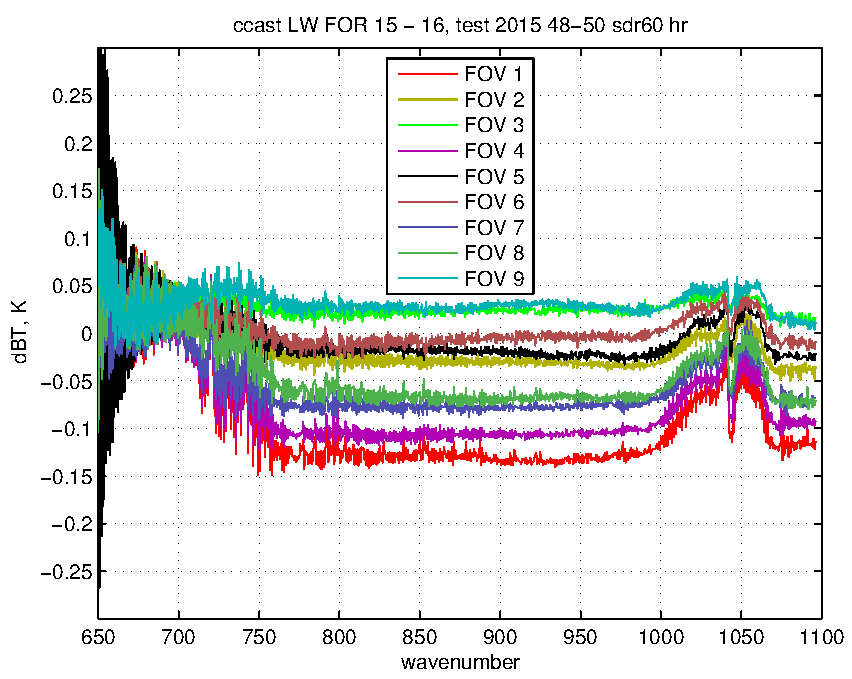
\includegraphics[scale=0.6]{figures/ccast_LW_sdif_2015_48-50_sdr60_hr.pdf}

ccast LW FOR 15 minus FOR 16, for the three-day test

\end{center}
\end{frame}
%----------- slide --------------------------------------------------%
\begin{frame}
\frametitle{sweep differences}
\begin{center}
  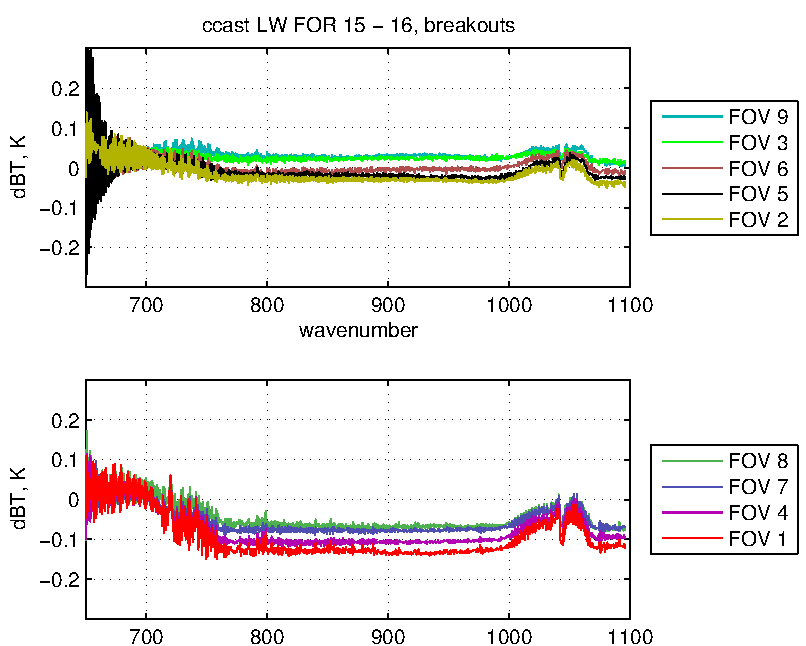
\includegraphics[scale=0.6]{figures/ccast_LW_sbrk_2015_48-50_sdr60_hr.pdf}

breakout of differences ordered by mid-band value

\end{center}
\end{frame}
%----------- slide --------------------------------------------------%
\begin{frame}
\frametitle{sweep differences}
\begin{center}
  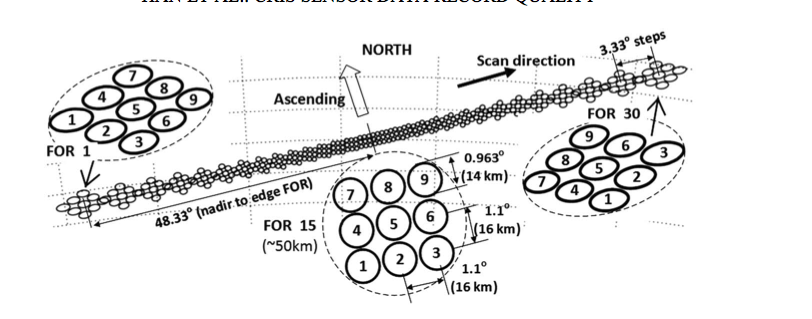
\includegraphics[scale=0.6]{figures/cris_FOR.png}
\end{center}
\cris\ near-nadir FOR positions from the ATBD.  Note that the two
FOV groups [9, 3, 6, 5, 2] and [8, 7, 4, 1] from the previous slide
approximately bisect this pattern
\end{frame}
%----------- slide --------------------------------------------------%
\begin{frame}
\frametitle{double difference}
\begin{center}
  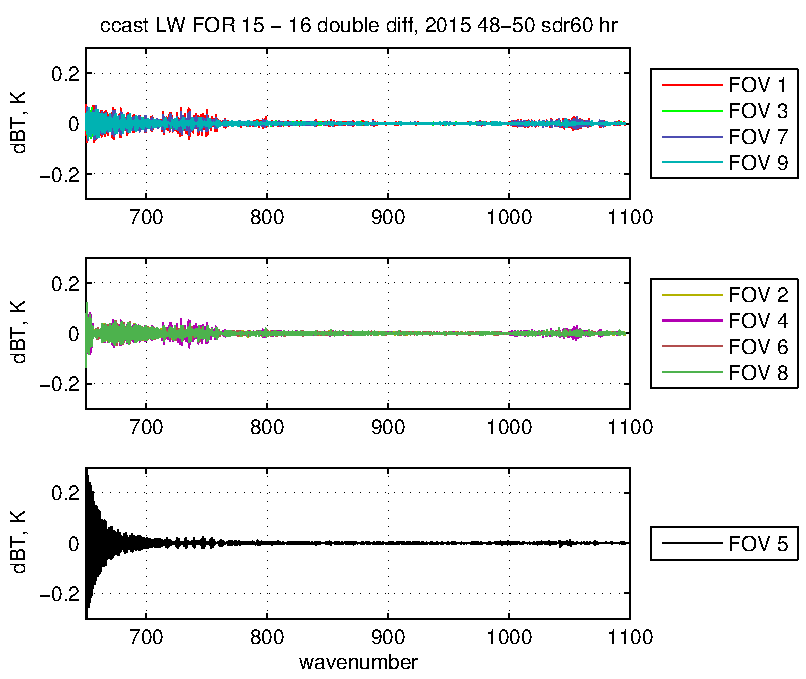
\includegraphics[scale=0.6]{figures/ccast_LW_sfil_2015_48-50_sdr60_hr.pdf}

(FOR 15 minus 16) minus convolved (FOR 15 minus 16)

\end{center}
\end{frame}
%----------- slide --------------------------------------------------%
\end{document}

